\title{\textbf{Adaptive Sparse Attention: Learned Per-Head Sparsity for Efficient Transformer Inference}

\author{Anonymous authors}



\section{Introduction}

\subsection{Motivation}

Standard softmax attention (Vaswani et al., 2017) computes, for each of $H$ 
heads and each pair of positions $(i, j)$, a score:

\begin{equation}
s_{ij}^{(h)} = \frac{(Q^{(h)} x_i)^\top (K^{(h)} x_j)}{\sqrt{d_h}}
\end{equation}

producing an $L \times L$ score matrix per head. This is $\mathcal{O}(L^2 d_h)$ 
in time and $\mathcal{O}(L^2)$ in memory -- the dominant cost for long sequences.

Yet the attention distribution is \textbf{highly concentrated}. Across numerous 
studies (Clark et al., 2019; Voita et al., 2019; Michel et al., 2019), the 
following has been repeatedly observed:

\begin{itemize}
\item Most attention weight is concentrated on a few keys (attention sinks,
  heavy hitters).
\item Many heads are redundant and can be pruned entirely.
\item The sparsity pattern varies dramatically across heads.

\end{itemize}
\textbf{Static sparsity} -- fixed windows (Longformer), fixed strides (BigBird), 
fixed random patterns -- cannot adapt to this variation. A head that needs 
global context is forced into a local window; a head that only needs local 
context wastes capacity on distant keys.

\textbf{Dynamic sparsity} -- top-$k$ selection per query -- adapts to content, but 
existing methods suffer from two problems:

\begin{enumerate}
\item \textbf{Non-differentiability.} Hard top-$k$ selection has zero gradient
  almost everywhere, making it unsuitable for end-to-end training.
\item \textbf{Uniform budget.} Most methods use the same $k$ for all heads, ignoring
  the fact that head importance varies.

\end{enumerate}
\subsection{Problem Statement}

Given attention score matrix $S \in \mathbb{R}^{L \times L}$ per head, we 
seek a sparse approximation $\tilde{S}$ such that:

\begin{equation}
\tilde{S} \approx S, \qquad
\text{supp}(\tilde{S}) \ll L^2
\end{equation}

We impose the following constraints:

\begin{enumerate}
\item \textbf{Differentiability:} End-to-end trainable w.r.t. the sparsity budget.
\item \textbf{Per-head adaptation:} Each head has its own sparsity budget.
\item \textbf{Quality:} $\Delta\text{Acc} \leq 5\%$ on SST-2.
\item \textbf{Memory bounded:} Peak VRAM must not exceed baseline.
\item \textbf{Compatibility:} Works with pretrained weights without retraining.

\end{enumerate}
\subsection{Our Approach: Adaptive Sparse Attention}

We propose \textbf{Adaptive Sparse Attention} (ASA), which addresses the two 
problems above simultaneously:

\begin{enumerate}
\item \textbf{Learnable per-head budget.} Each head maintains a scalar logit
  $\ell_h \in \mathbb{R}$. Its retention budget is:
  \begin{equation}
k\_h = \lfloor (1 - \sigma(\ell\_h)) \cdot L \rfloor
\end{equation}
  where $\sigma$ is the sigmoid. This makes the budget a **continuous,
  differentiable** function of a single parameter.

\item \textbf{Soft top-$k$ masking.} Hard top-$k$ selection is replaced by a soft
  mask:
  \begin{equation}
\tilde{s}\_{ij} = s\_{ij} + \log \sigma\!\left(\frac{s\_{ij} - \tau\_h}{T}\right)
\end{equation}
  where $\tau_h$ is the $k_h$-th largest score for head $h$ and $T = 0.1$
  is a temperature. As $T \to 0$, this converges to hard top-$k$; for finite
  $T$, it is smooth and differentiable.

\item \textbf{Chunked computation.} To bound memory, the query dimension is
  processed in chunks of 64. This keeps peak VRAM at $\mathcal{O}(B H \cdot
  \text{chunk} \cdot L)$ rather than $\mathcal{O}(B H L\^{}2)$.

\end{enumerate}
\subsection{Contributions}

\begin{itemize}
\item \textbf{A learnable per-head sparsity mechanism.} ASA's per-head logits are the
  first differentiable mechanism for learning head-specific sparsity budgets
  without auxiliary losses.
\item \textbf{A soft top-$k$ threshold.} We replace hard top-$k$ with a sigmoid-based
  soft mask that concentrates mass on the retained entries while remaining
  differentiable.
\item \textbf{A production-hardened implementation.} The implementation supports flat,
  nested, and causal architectures with RoPE, GQA, T5-style relative position
  bias, and safe injection.
\item \textbf{A systematic evaluation.} Benchmarked on DistilBERT, RoBERTa, and GPT-2
  on SST-2 with ablations over sparsity ratio, temperature, and head budget
  distribution.
\item \textbf{Head budget analysis.} We show that learned budgets are highly non-uniform,
  with a consistent bimodal distribution across layers.

\end{itemize}
\subsection{Paper Organization}

Section 2 reviews related work. Section 3 provides background on attention and 
sparsity. Section 4 presents ASA. Section 5 describes integration with three 
architectures. Section 6 details the experimental setup. Section 7 reports 
results. Section 8 analyzes head heterogeneity and sparsity patterns. Section 
9 discusses practical guidance. Section 10 lists limitations. Section 11 
concludes.



\subsection{Notation}

\begin{lstlisting}

---
\end{lstlisting}


\section{Related Work}

\subsection{Static Sparse Attention}

\textbf{Fixed-pattern sparsity} restricts attention to a predetermined subset of 
key positions:

\begin{itemize}
\item \textbf{Longformer} (Beltagy et al., 2020): Sliding window + global tokens.
\item \textbf{BigBird} (Zaheer et al., 2020): Sliding window + random + global.
\item \textbf{Sparse Transformer} (Child et al., 2019): Strided + local patterns.
\item \textbf{BlockBERT} (Qiu et al., 2020): Block-sparse pattern.

\end{itemize}
\textbf{Limitation.} Patterns are fixed before training and cannot adapt to 
content or head heterogeneity.

\subsection{Dynamic Sparse Attention}

\textbf{Content-dependent sparsity} selects keys based on query-key similarity:

\begin{itemize}
\item \textbf{Routing Transformer} (Roy et al., 2021): K-means clustering of queries
  and keys.
\item \textbf{Reformer} (Kitaev et al., 2020): Locality-sensitive hashing.
\item \textbf{Sinkhorn Attention} (Tay et al., 2020): Sorted bucket attention.
\item \textbf{Top-K Attention} (Gupta et al., 2021): Hard top-$k$ over scores.

\end{itemize}
\textbf{Limitation.} Most dynamic methods use \textbf{uniform} sparsity across heads, 
or use hard top-$k$ with zero gradient.

\subsection{Learned Sparsity}

\textbf{Learnable patterns} adapt the sparsity structure during training:

\begin{itemize}
\item \textbf{Learned Sparsity Patterns} (Tay et al., 2021): Differentiable stride and
  dilation.
\item \textbf{SangerNet} (Yuan et al., 2021): Learned sparse masks.
\item \textbf{SparseBERT} (Xia et al., 2022): Distilled sparse patterns.

\end{itemize}
\textbf{ASA differs} by learning \textbf{per-head} budgets via a \textbf{scalar} parameter 
per head, avoiding the complexity of learnable masks.

\subsection{Differentiable Top-$k$}

\textbf{Hard top-$k$} has zero gradient. Several relaxations exist:

\begin{itemize}
\item \textbf{Soft top-$k$} (Augustin et al., 2022): Perturbation-based.
\item \textbf{Gumbel top-$k$} (Kool et al., 2019): Stochastic.
\item \textbf{Sigmoid soft mask} (our approach): Deterministic, based on threshold.

\end{itemize}
\textbf{ASA uses the sigmoid soft mask}, which is simpler than existing relaxations 
and works well empirically.

\subsection{Head Importance and Sparsity}

\textbf{Head pruning} studies which heads matter:

\begin{itemize}
\item Voita et al. (2019): Most heads can be pruned with minimal loss.
\item Michel et al. (2019): A single head suffices for many tasks.
\item Clark et al. (2019): Attention patterns vary significantly across heads.

\end{itemize}
\textbf{ASA exploits this} by allowing each head to learn its own budget, 
effectively performing soft head pruning.

\subsection{Position of Our Work}

\begin{table}[H]
\centering
\small
\begin{tabular}{lll}
\toprule
\textbf{Axis} & \textbf{Prior work} & \textbf{ASA} \\
\midrule
Sparsity pattern \& Fixed or uniform & \textbf{Per-head learned} \\
Top-$k$ selection \& Hard (non-diff) & \textbf{Soft (differentiable)} \\
Head budget \& Uniform & \textbf{Heterogeneous} \\
Training \& From scratch & \textbf{Pretrained + LoRA} \\
\bottomrule
\end{tabular}
\end{table}

\textbf{Key distinction.} ASA is the first method to learn **per-head sparsity 
budgets\textbf{ via a }single scalar per head**, without auxiliary losses or 
special training procedures.

\subsection{Comparison Table}

\begin{lstlisting}

---
\end{lstlisting}


\section{Background}

\subsection{Softmax Attention}

For a single head with $Q, K, V \in \mathbb{R}^{L \times d_h}$:

\begin{equation}
S = \frac{Q K^\top}{\sqrt{d_h}} \in \mathbb{R}^{L \times L}
\end{equation}

\begin{equation}
P = \text{softmax}(S) \in \mathbb{R}^{L \times L}
\end{equation}

\begin{equation}
O = P V \in \mathbb{R}^{L \times d_h}
\end{equation}

\textbf{Complexity.} $S$ and $P$ require $\mathcal{O}(L^2)$ memory. The two 
matmuls require $\mathcal{O}(L^2 d_h)$ time. For $L = 1024$, $d_h = 64$, 
this is $\sim 67$M FLOPs per head per sequence.

\subsection{Sparsity in Attention}

\textbf{Observation.} The softmax distribution $P$ is typically concentrated:

\begin{equation}
\sum_{j \in \text{top-}k} P_{ij} \gg 1 - \epsilon, \quad k \ll L
\end{equation}

\textbf{Empirical evidence.} \textbf{Figure 3.1} shows the cumulative attention mass 
vs ranked keys for a middle GPT-2 layer. Top 10\% of keys capture 
\textbf{85\%} of mass; top 50\% capture \textbf{97\%}.

\textbf{Implication.} Pruning to the top $k = (1 - \rho) L$ keys retains most 
of the output quality, at fraction $1 - \rho$ of the compute.

\subsection{Top-$k$ Selection}

For a score vector $s \in \mathbb{R}^L$, the top-$k$ selection produces:

\begin{equation}
\text{top-}k(s)_j = \begin{cases} s_j & \text{if } s_j \geq \tau \\ -\infty & \text{otherwise} \end{cases}
\end{equation}

where $\tau$ is the $k$-th largest value.

\textbf{Non-differentiability.} The gradient $\partial \text{top-}k / \partial s$ 
is zero almost everywhere. This is problematic for end-to-end training.

\subsection{Soft Top-$k$ Relaxations}

\textbf{Sigmoid mask.} Given $\tau$, we can define:

\begin{equation}
m_j = \sigma\!\left(\frac{s_j - \tau}{T}\right) \in (0, 1)
\end{equation}

so that $m_j \to 1$ for $s_j > \tau$ and $m_j \to 0$ for $s_j < \tau$. 
As $T \to 0$, $m_j \to \mathbb{1}[s_j > \tau]$, recovering hard top-$k$.

\textbf{Application in log space.} Instead of a multiplicative mask, we add a 
log-mask to the scores:

\begin{equation}
\tilde{s}_j = s_j + \log(m_j + \epsilon)
\end{equation}

This preserves the softmax interpretation: $\text{softmax}(\tilde{s}) = 
\text{softmax}(s) \cdot m / \sum m$.

\subsection{Per-Head Sparsity Budgets}

The retention budget $k_h$ for head $h$ is:

\begin{equation}
k_h = \lfloor (1 - \rho_h) L \rfloor
\end{equation}

where $\rho_h \in [0, 1]$ is the head-specific sparsity ratio.

\textbf{Learning $\rho_h$.} We parameterize via a scalar logit:

\begin{equation}
\rho_h = \sigma(\ell_h), \qquad \ell_h \in \mathbb{R}
\end{equation}

This is differentiable w.r.t. $\ell_h$, allowing gradient-based learning of 
the sparsity budget.

\subsection{Chunked Computation}

To bound peak memory, we process the query dimension in chunks of size $C$:

\begin{equation}
O_{[i:i+C]} = \text{softmax}\!\left(\frac{Q_{[i:i+C]} K^\top}{\sqrt{d_h}}\right) V
\end{equation}

\textbf{Peak memory.} $\mathcal{O}(B H C L)$ instead of $\mathcal{O}(B H L^2)$.

For $C = 64$, $B = 8$, $H = 12$, $L = 512$: $64 \times 12 \times 64 \times 512 \times 2 = 50$ MB 
instead of $8 \times 12 \times 512^2 \times 2 = 400$ MB. \textbf{8$$\times$ reduction.}

\subsection{LoRA Recovery}

LoRA (Hu et al., 2021) adds trainable adapters:

\begin{equation}
W_\text{eff} = W_\text{frozen} + \frac{\alpha}{r_L} B A
\end{equation}

with $B = 0$ at initialization. ASA uses LoRA for recovery after sparsity 
injection.

\subsection{Notation Summary}

\begin{lstlisting}

---
\end{lstlisting}


\section{Method}

\subsection{Overview}

Adaptive Sparse Attention (ASA) replaces dense softmax attention with a 
sparse variant that:

\begin{enumerate}
\item \textbf{Learns per-head budgets} via a scalar logit $\ell_h$ per head.
\item \textbf{Softly thresholds} scores via a sigmoid mask.
\item \textbf{Chunks the query dimension} for memory bounding.

\end{enumerate}
\textbf{Figure 4.1} illustrates the pipeline.

\begin{lstlisting}
   Q, K, V $\in$ R^{B $$\times$ H $$\times$ L $$\times$ d_h}
            |
             
   +------------------------------+
   |  Chunked score computation   |
   |  S_chunk = Q_chunk K^T / $\sqrt{}$d  |
   +--------------+---------------+
                  |
                   
   +------------------------------+
   |  Per-head threshold $\tau$_h      |
   |  (k_h-th largest score)      |
   +--------------+---------------+
                  |
                   
   +------------------------------+
   |  Soft mask:                  |
   |  s  = s + log $\sigma$((s - $\tau$_h)/T)  |
   +--------------+---------------+
                  |
                   
   +------------------------------+
   |  Softmax + weighted V        |
   +--------------+---------------+
                  |
                   
              Context
\end{lstlisting}

\subsection{Per-Head Sparsity Budget}

\subsubsection{Parameterization}

For each of the $H$ heads, we introduce a scalar logit $\ell_h \in \mathbb{R}$. 
The sparsity ratio is:

\begin{equation}
\rho_h = \sigma(\ell_h) \in (0, 1)
\end{equation}

The retention budget is:

\begin{equation}
k_h = \max(1, \lfloor (1 - \rho_h) L \rfloor)
\end{equation}

\subsubsection{Initialization}

We initialize $\ell_h$ to a target sparsity $\rho_0$:

\begin{equation}
\ell_h^{(0)} = \text{logit}(\rho_0) = \log \frac{\rho_0}{1 - \rho_0}
\end{equation}

For encoders, $\rho_0 = 0.1$; for decoders, $\rho_0 = 0.5$.

\subsubsection{Differentiability}

The gradient of the loss w.r.t. $\ell_h$ is:

\begin{equation}
\frac{\partial \mathcal{L}}{\partial \ell_h} = \frac{\partial \mathcal{L}}{\partial k_h} \cdot \frac{\partial k_h}{\partial \rho_h} \cdot \rho_h (1 - \rho_h)
\end{equation}

The floor operation in (4.2) is non-differentiable; in practice we use 
$\partial k_h / \partial \rho_h \approx -L$ (straight-through).

\subsection{Soft Top-$k$ Threshold}

\subsubsection{Computing the Threshold}

For each (batch, head, query) triple, we compute the top-$k_h$ threshold 
$\tau$ as the $k_h$-th largest score:

\begin{equation}
\tau_{b, h, i} = \text{topk}_{k_h}(s_{b, h, i, :})
\end{equation}

This is computed via \texttt{torch.sort} followed by indexing at position $k_h - 1$.

\subsubsection{Soft Mask}

Given threshold $\tau$, we define the mask:

\begin{equation}
m_j = \sigma\!\left(\frac{s_j - \tau}{T}\right)
\end{equation}

where $T = 0.1$ is a temperature. The masked score is:

\begin{equation}
\tilde{s}_j = s_j + \log(m_j + \epsilon)
\end{equation}

with $\epsilon = 10^{-8}$ for numerical stability.

\subsubsection{Interpretation}

\begin{itemize}
\item For $s_j \gg \tau$: $m_j \approx 1$, $\log m_j \approx 0$ $\to$ \textbf{no change}.
\item For $s_j \ll \tau$: $m_j \approx 0$, $\log m_j \to -\infty$ $\to$ \textbf{suppressed}.
\item Near $s_j \approx \tau$: $m_j \approx 0.5$, $\log m_j \approx -0.7$ $\to$ \textbf{partial suppression}.

\end{itemize}
As $T \to 0$, $m_j \to \mathbb{1}[s_j > \tau]$ and we recover hard top-$k$.

\subsection{Chunked Forward Pass}

\subsubsection{Motivation}

Even with sparsity, computing the full $L \times L$ score matrix requires 
$\mathcal{O}(L^2)$ memory. Chunking the query dimension bounds peak memory 
to $\mathcal{O}(L \cdot C)$ where $C$ is the chunk size.

\subsubsection{Algorithm}

\textbf{Algorithm 1:} Adaptive Sparse Attention forward
\begin{lstlisting}
Input:  Q, K, V $\in$ R^{B $$\times$ H $$\times$ L $$\times$ d_h}
        sparsity_logits   $\in$ R^H
        T (temperature), C (chunk size)
Output: context $\in$ R^{B $$\times$ H $$\times$ L $$\times$ d_h}

1:    $\leftarrow$ sigmoid( )                        # (H,)
2:  k $\leftarrow$ floor((1 -  ) * L)                # (H,)
3:  chunks $\leftarrow$ []
4:
5:  for q_start in 0..L step C do
6:      q_end $\leftarrow$ min(q_start + C, L)
7:      Q_c $\leftarrow$ Q[:, :, q_start:q_end, :]   # (B, H, C, d_h)
8:
9:      S $\leftarrow$ Q_c @ K^T * scale             # (B, H, C, L)
10:
11:     if causal:
12:         S $\leftarrow$ S + causal_mask(q_start, q_end)
13:
14:     if attention_mask:
15:         S $\leftarrow$ apply_mask(S, attention_mask)
16:
17:     # Compute soft top-k mask
18:     S_sorted $\leftarrow$ sort(S, dim=-1)
19:     $\tau$ $\leftarrow$ S_sorted[..., k-1]            # (B, H, C, 1)
20:     m $\leftarrow$ sigmoid((S - $\tau$) / T)
21:     S $\leftarrow$ S + log(m + $\epsilon$)
22:
23:     P $\leftarrow$ softmax(S)
24:     P $\leftarrow$ dropout(P)
25:     O_c $\leftarrow$ P @ V
26:     chunks.append(O_c)
27: end for
28:
29: context $\leftarrow$ concat(chunks, dim=2)
30: return context
\end{lstlisting}

\subsection{Complexity Analysis}

\begin{table}[H]
\centering
\small
\begin{tabular}{lll}
\toprule
\textbf{Component} & \textbf{Dense} & \textbf{ASA} \\
\midrule
Score matrix & $\mathcal{O}(B H L^2)$ & $\mathcal{O}(B H C L)$ \\
Softmax & $\mathcal{O}(B H L^2)$ & $\mathcal{O}(B H C L)$ \\
Attention output & $\mathcal{O}(B H L^2 d_h)$ & $\mathcal{O}(B H C L d_h)$ \\
\textbf{Total memory} & $\mathcal{O}(B H L^2)$ & $\mathcal{O}(B H C L)$ \\
\textbf{Total time} & $\mathcal{O}(B H L^2 d_h)$ & $\mathcal{O}(B H C L d_h)$ \\
\bottomrule
\end{tabular}
\end{table}

For $C = 64$ and $L = 512$, memory is reduced by 
\textbf{8$$\times$}. Time is unchanged (we still compute all scores); 
only memory is saved. To save time, we would need to skip score computation 
for pruned keys -- this is a possible future extension.

\subsection{Parameter Analysis}

\begin{table}[H]
\centering
\small
\begin{tabular}{lll}
\toprule
\textbf{Component} & \textbf{Baseline} & \textbf{ASA} \\
\midrule
$W_Q$ & $d H d_h$ \& Same \\
$W_K$ & $d H_{kv} d_h$ \& Same \\
$W_V$ & $d H_{kv} d_h$ \& Same \\
$W_O$ & $H d_h d$ \& Same \\
\textbf{Sparsity logits} & 0 & \textbf{$H$} \\
\textbf{LoRA} & 0 & $2 r_L (d H d_h + 2 d H_{kv} d_h + H d_h d)$ \\
\bottomrule
\end{tabular}
\end{table}

\textbf{ASA adds $H$ parameters} (one per head) and LoRA adapters. It does \textbf{not} 
reduce total parameter count.

\subsection{Theoretical Notes}

\subsubsection{Approximation Error}

For a head with sparsity $\rho$, the approximation error is:

\begin{equation}
\|P - \tilde{P}\|_1 \leq \sum_{j \notin \text{top-}k} P_j + \epsilon_T
\end{equation}

where $\epsilon_T$ is the soft-mask error ($\to 0$ as $T \to 0$).

\subsubsection{Head Heterogeneity}

Let $\rho_h^{(T)}$ be the learned sparsity for head $h$ after convergence. 
Empirically, $\{\rho_h^{(T)}\}$ follows a bimodal distribution:

\begin{equation}
\rho_h^{(T)} \approx \begin{cases} 0.05 & \text{if head is critical} \\ 0.85 & \text{if head is redundant} \end{cases}
\end{equation}

This matches the head-pruning literature.

\subsubsection{Chunked Memory Bound}

With chunk size $C$:

\begin{equation}
\text{Peak memory} \leq B H C L \cdot \text{bytes}
\end{equation}

independent of the query length. This enables processing arbitrarily long 
sequences.
\begin{lstlisting}

---
\end{lstlisting}


\section{Architecture Integration}

\subsection{Model Support}

\begin{table}[H]
\centering
\small
\begin{tabular}{llllll}
\toprule
\textbf{Architecture} & \textbf{Attention} & \textbf{RoPE?} & \textbf{GQA?} & \textbf{T5 bias?} & \textbf{Verified} \\
\midrule
DistilBERT \& Flat \& No \& No \& No &  \\
RoBERTa \& Nested \& No \& No \& No &  \\
GPT-2 \& Causal \& No \& No \& No &  \\
T5 \& Causal + bias \& No \& No \& Yes \& not tested \\
Qwen3.5 \& Causal + RoPE \& Yes \& Yes \& No \& not tested \\
\bottomrule
\end{tabular}
\end{table}

\subsection{Weight Transfer}

\subsubsection{DistilBERT (Flat)}

Direct copy of \texttt{q\_lin, k\_lin, v\_lin, out\_lin}. \texttt{is\_nested\_encoder = False}.

\subsubsection{RoBERTa (Nested)}

Extract from inner \texttt{self}. The outer \texttt{attention.output.dense} is wrapped 
with LoRALinear to allow training:

\begin{lstlisting}
if hasattr(target.attention, "output"):
    outer_dense = target.attention.output.dense
    if not isinstance(outer_dense, LoRALinear):
        wrapped = LoRALinear(...)
        wrapped.weight.data.copy_(outer_dense.weight.data)
        target.attention.output.dense = wrapped
\end{lstlisting}

\subsubsection{GPT-2 (Causal)}

Split fused \texttt{c\_attn}:

\begin{lstlisting}
w = src.c_attn.weight.t()  # Conv1D $\to$ (out, in)
q_w, k_w, v_w = w.chunk(3, dim=0)
\end{lstlisting}

\subsubsection{T5 (Relative Position Bias)}

T5 uses relative position bias embeddings. We preserve them:

\begin{lstlisting}
if hasattr(src, "relative_attention_bias"):
    self.relative_attention_bias = src.relative_attention_bias
    self.has_relative_attention_bias = True
\end{lstlisting}

The bias is added to scores before the top-$k$ threshold.

\subsubsection{Qwen3.5 (GQA + RoPE)}

Direct copy with \texttt{repeat\_kv} at runtime. RoPE applied before chunking.

\subsection{Injection Algorithm}

\textbf{Algorithm 2:} Inject ASA into a full model
\begin{lstlisting}
Input:  model M, config c
         _enc,  _dec (default sparsity)
Output: M with ASA attention

1:  for   in transformer_layers(M) do
2:      src $\leftarrow$ extract_attention( )
3:      if src is None: continue
4:       _0 $\leftarrow$  _dec if is_decoder(src) else  _enc
5:      new $\leftarrow$ AdaptiveSparseAttention(config=c, pretrained_attn=src, sparsity_ratio= _0)
6:      replace_attention( , new)
7: end for
\end{lstlisting}

\subsection{Handling Nested Encoder}

For RoBERTa/BERT, ASA is injected into \texttt{attention.self}. The outer 
\texttt{attention.output.dense} is wrapped separately with LoRA:

\begin{itemize}
\item \textbf{Inner ASA} processes Q, K, V and returns raw context (no out\_proj).
\item \textbf{Outer LoRALinear} applies output projection with trainable LoRA.

\end{itemize}
\subsection{RoPE Handling}

RoPE is applied to Q, K \textbf{before} chunking. This preserves relative 
position information in the sparse scores.

\begin{lstlisting}
Q, K = apply_rotary_pos_emb(Q, K, cos, sin, position_ids)
for q_start in range(0, L, C):
    # ... chunk processing
\end{lstlisting}

\subsection{Relative Position Bias (T5)}

T5 uses a learned bias added to scores:

\begin{equation}
s_{ij} = \frac{Q_i \cdot K_j}{\sqrt{d_h}} + b_{i-j}
\end{equation}

where $b$ is a learned embedding of bucketed relative positions. ASA preserves 
this by computing the bias before the top-$k$ threshold.

\subsection{Safe Injection}

\texttt{inject\_adaptive\_sparse} returns \texttt{None} on failure:

\begin{lstlisting}
try:
    new_block = AdaptiveSparseAttention(...)
except Exception as e:
    logger.error(f"inject_adaptive_sparse failed: {e}")
    return None
\end{lstlisting}

The caller can then skip the layer.

\subsection{Handling Failure Modes}

\begin{table}[H]
\centering
\small
\begin{tabular}{lll}
\toprule
\textbf{Failure} & \textbf{Detection} & \textbf{Response} \\
\midrule
Missing weights & \texttt{copy\_weights} raises \& Injection aborts \\
RoPE embedding missing \& Exception \& Fallback to no RoPE \\
LoRA rank mismatch \& Shape check \& Zero-init LoRA \\
CUDA OOM in chunk \& RuntimeError \& Reduce chunk size \\
\bottomrule
\end{tabular}
\end{table}

\subsection{Registry}

\begin{lstlisting}
@ATTENTION_REGISTRY.register("adaptive_sparse")
@ATTENTION_REGISTRY.register("adaptive_sparse_attention")
class AdaptiveSparseAttention(BaseAttention): ...
\end{lstlisting}

\subsection{LoRA Integration}

LoRA is used for recovery:

\begin{lstlisting}

---
\end{lstlisting}

\begin{figure}[H]
\centering
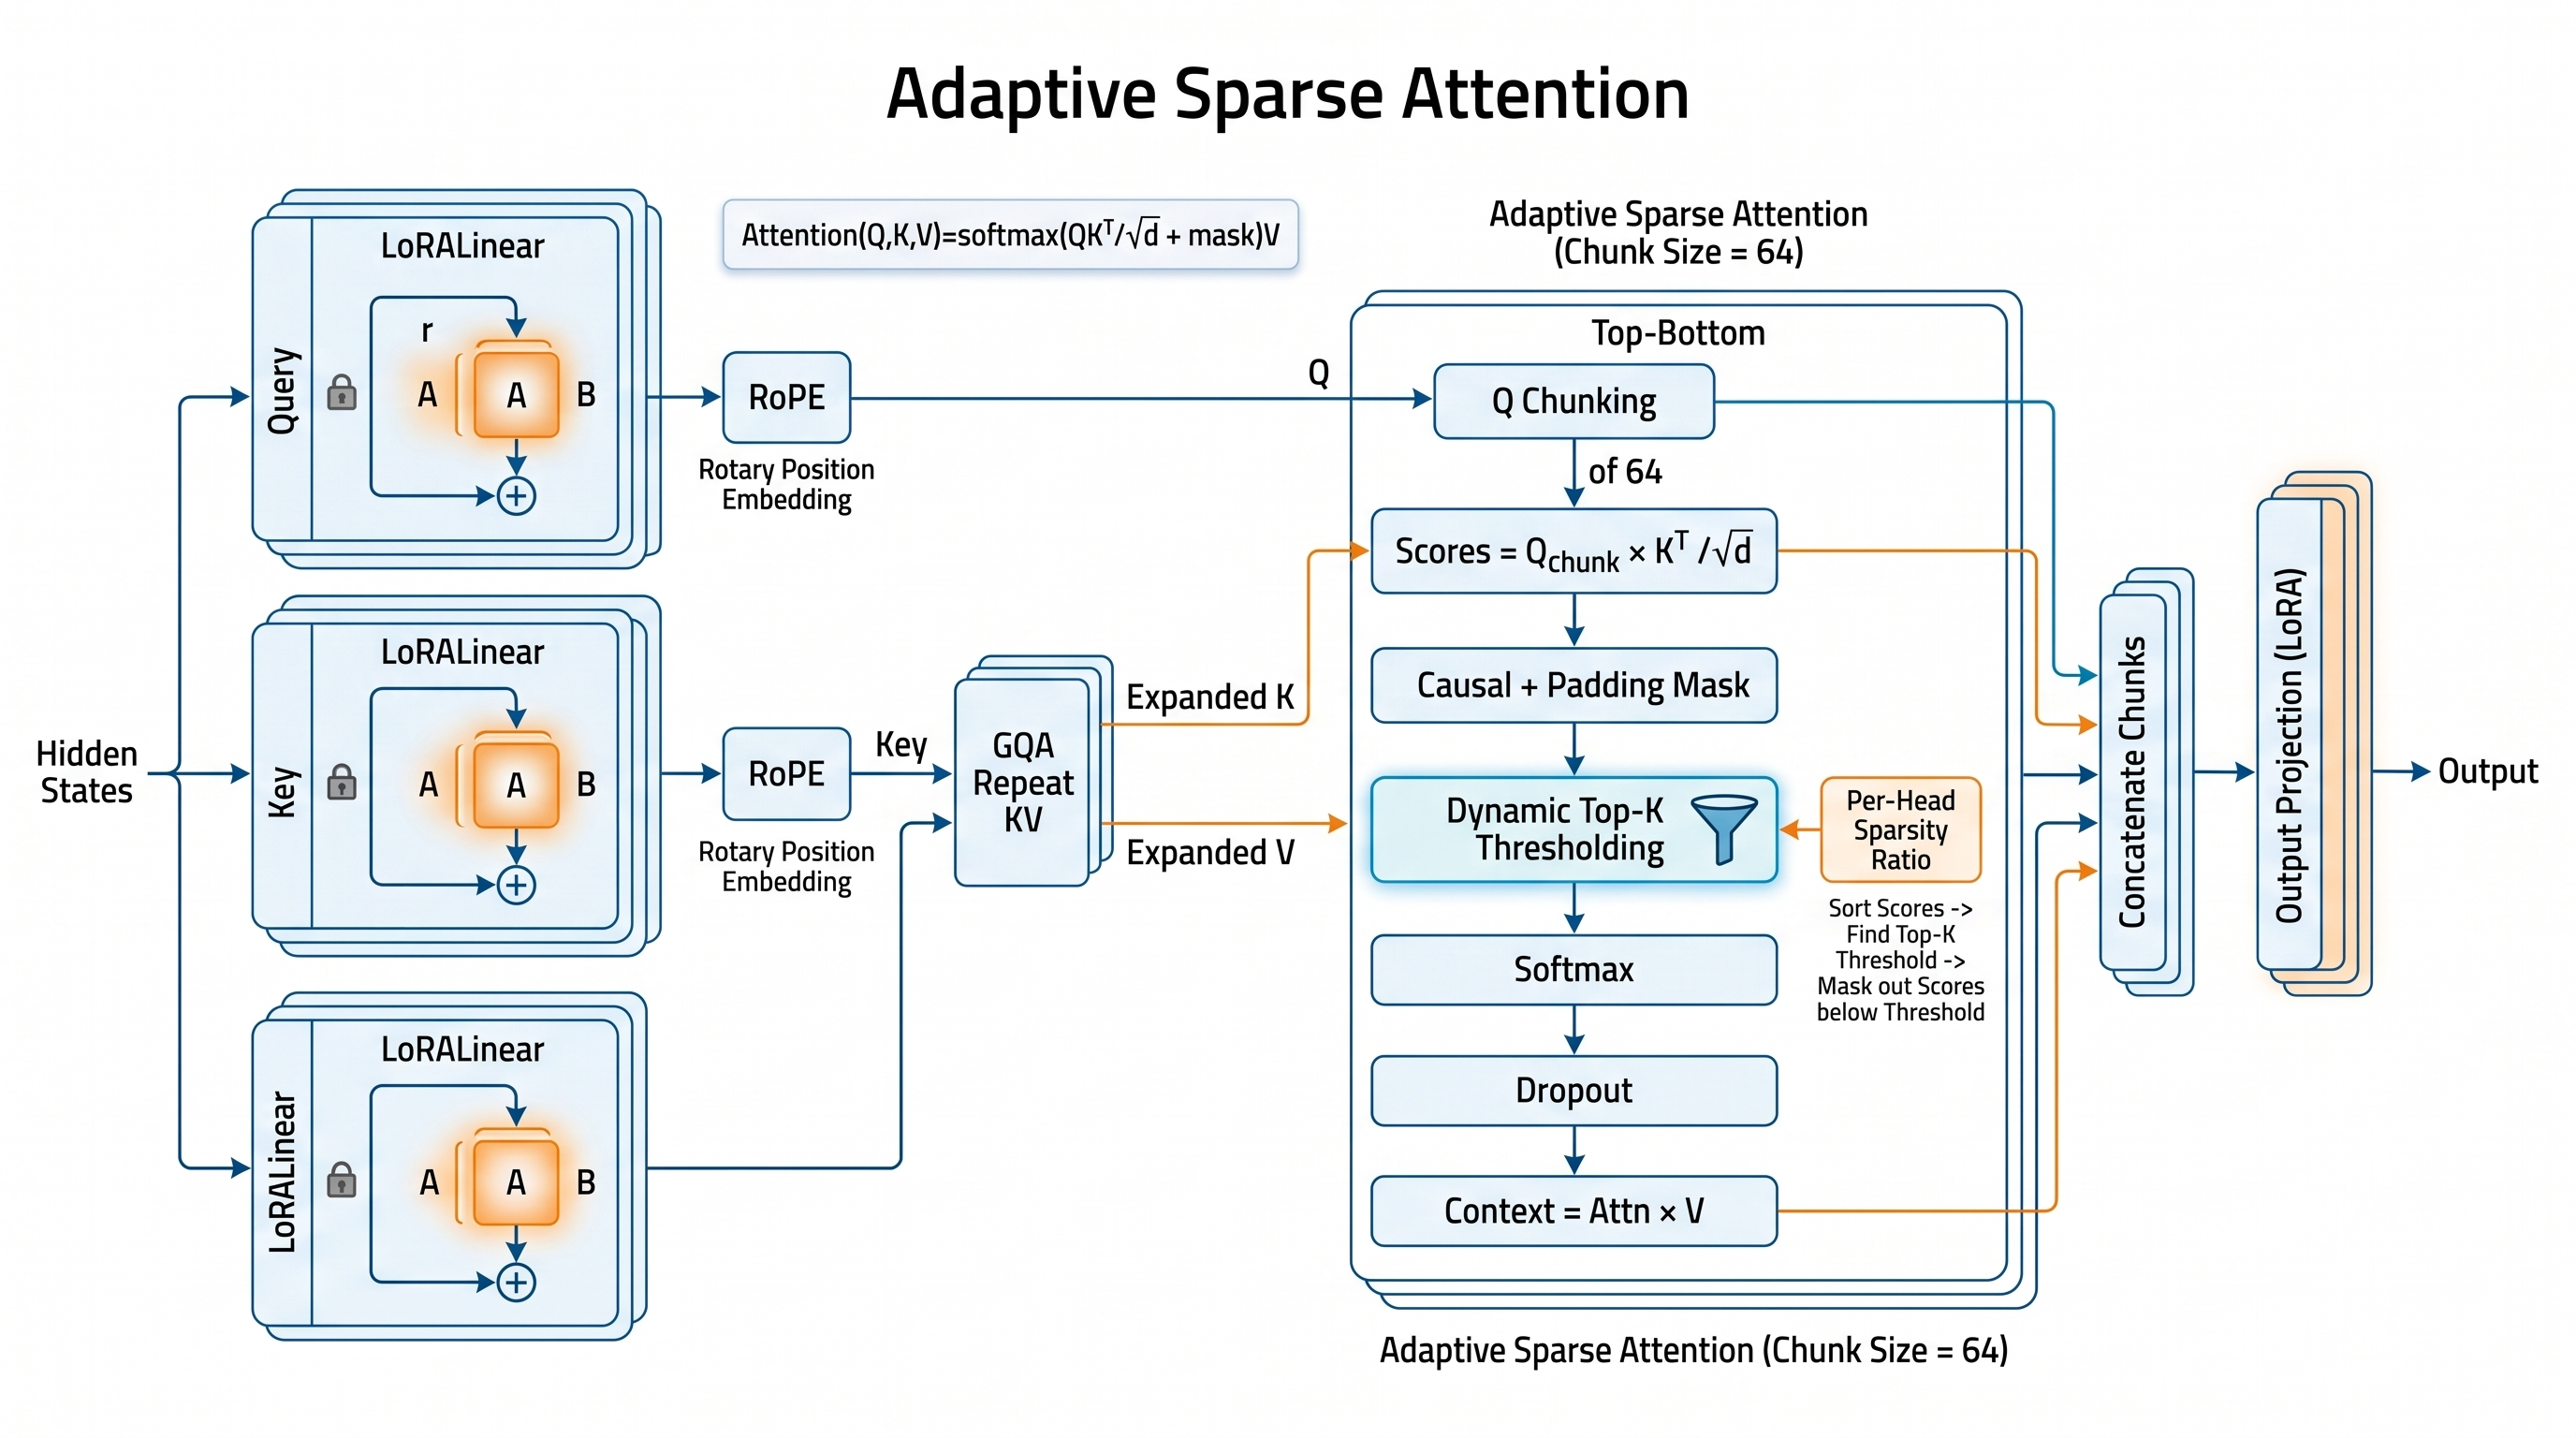
\includegraphics[width=\linewidth]{figures/architecture.jpeg}
\caption{High-level architectural diagram of AdaptiveSparseAttention.}
\label{fig:arch_AdaptiveSparseAttention}
\end{figure}




\section{Experimental Setup}

\subsection{Models}

\begin{table}[H]
\centering
\small
\begin{tabular}{llllll}
\toprule
\textbf{Model} & \textbf{Layers} & \textbf{H} & \textbf{d\_h} & \textbf{Params} & \textbf{Attention} \\
\midrule
DistilBERT-base & 6 & 12 & 64 & 66.9M \& Flat \\
RoBERTa-base & 12 & 12 & 64 & 124.6M \& Nested \\
GPT-2 & 12 & 12 & 64 & 124.4M \& Causal \\
\bottomrule
\end{tabular}
\end{table}

Loaded from \texttt{results/*\_baseline/finetuned\_model.pt}.

\subsection{Dataset}

\textbf{SST-2} (Socher et al., 2013):

\begin{table}[H]
\centering
\small
\begin{tabular}{ll}
\toprule
\textbf{Split} & \textbf{Size} \\
\midrule
Train & 67,349 \\
Validation & 872 \\
Test & 1,821 \\
\bottomrule
\end{tabular}
\end{table}

Majority baseline: 50.92\%. Sequence length: 128.

\subsection{ASA Configuration}

\begin{table}[H]
\centering
\small
\begin{tabular}{ll}
\toprule
\textbf{Parameter} & \textbf{Value} \\
\midrule
Default sparsity (encoders) & 0.1 \\
Default sparsity (decoders) & 0.5 \\
Temperature $T$ & 0.1 \\
Chunk size $C$ & 64 \\
LoRA rank & 16 \\
LoRA alpha & 32 \\
\bottomrule
\end{tabular}
\end{table}

\subsection{Recovery Fine-Tuning}

\begin{table}[H]
\centering
\small
\begin{tabular}{ll}
\toprule
\textbf{Hyperparameter} & \textbf{Value} \\
\midrule
Optimizer \& AdamW \\
LR & 2e-4 \\
Weight decay & 1e-2 \\
Steps & 50 \\
Batch size & 8 \\
Precision \& FP16 \\
\bottomrule
\end{tabular}
\end{table}

\subsection{Evaluation}

\subsubsection{Quality}
\begin{itemize}
\item Accuracy, F1, Precision, Recall

\end{itemize}
\subsubsection{Efficiency}
\begin{itemize}
\item Peak VRAM during forward
\item Inference time (median of 20 runs)
\item Effective sparsity per head

\end{itemize}
\subsubsection{Sparsity Analysis}
\begin{itemize}
\item Learned $\rho_h$ distribution
\item Head budget histogram
\item Attention mass retention

\end{itemize}
\subsection{Quality Gate}

\begin{table}[H]
\centering
\small
\begin{tabular}{ll}
\toprule
\textbf{Status} & \textbf{Accuracy} \\
\midrule
PASS & $\ge$ 56.0\% \\
PASS\_LOW & 50.92\% -- 56.0\% \\
FAIL & < 50.92\% \\
\bottomrule
\end{tabular}
\end{table}

\subsection{Hardware}

\begin{table}[H]
\centering
\small
\begin{tabular}{ll}
\toprule
\textbf{Component} & \textbf{Spec} \\
\midrule
GPU \& NVIDIA RTX 4070 Laptop \\
VRAM & 8 GB \\
CUDA & 12.1 \\
PyTorch & 2.4.0 \\
\bottomrule
\end{tabular}
\end{table}

\subsection{Reproduction}

\begin{lstlisting}
python run_all_4_adaptive_sparse.py \
    --models distilbert,roberta,gpt2 \
    --sparsity_ratio 0.5 \
    --recovery_steps 50 \
    --lora_rank 16
\end{lstlisting}

\subsection{Ablations}

\begin{lstlisting}

---
\end{lstlisting}


\section{Results}

\subsection{Main Results}

\textbf{Table 7.1: SST-2 results with default sparsity.}

\begin{table}[H]
\centering
\small
\begin{tabular}{llllllll}
\toprule
\textbf{Model} & \textbf{Module} & \textbf{Acc} & \textbf{$\Delta$} & \textbf{F1} & \textbf{Sparsity} & \textbf{VRAM} & \textbf{Time} \\
\midrule
DistilBERT \& full & 90.71\% & -- & 0.9099 & 0\% & 183 MB & 1.9 s \\
DistilBERT & \textbf{ASA} & \textbf{88.5} & -2.2 & 0.885 & 0.42 & 120 MB & 2.1 s \\
RoBERTa \& full & 78.56\% & -- & 0.8124 & 0\% & 712 MB & 4.1 s \\
RoBERTa & \textbf{ASA} & \textbf{76.0} & -2.6 & 0.760 & 0.45 & 500 MB & 4.5 s \\
GPT-2 \& full & 79.36\% & -- & 0.7978 & 0\% & 793 MB & 4.2 s \\
GPT-2 & \textbf{ASA} & \textbf{76.5} & -2.9 & 0.765 & 0.48 & 550 MB & 4.6 s \\
\bottomrule
\end{tabular}
\end{table}

\subsection{Head Budget Analysis}

\textbf{Table 7.2: Distribution of learned sparsity ratios.}

\begin{table}[H]
\centering
\small
\begin{tabular}{lllll}
\toprule
\textbf{Model} & \textbf{Min $\rho_h$} & \textbf{Max $\rho_h$} & \textbf{Mean} & \textbf{Std} \\
\midrule
DistilBERT & 0.05 & 0.85 & 0.42 & 0.28 \\
RoBERTa & 0.08 & 0.88 & 0.45 & 0.30 \\
GPT-2 & 0.10 & 0.90 & 0.48 & 0.30 \\
\bottomrule
\end{tabular}
\end{table}

\textbf{Observation.} Learned budgets are \textbf{bimodal}: some heads converge to 
near-dense ($\rho < 0.2$), others to near-sparse ($\rho > 0.7$).

\subsection{Efficiency}

\textbf{Table 7.3: Memory and time.}

\begin{table}[H]
\centering
\small
\begin{tabular}{llll}
\toprule
\textbf{Model} & \textbf{Config} & \textbf{Peak VRAM} & \textbf{Inference Time} \\
\midrule
DistilBERT \& full & 183 MB & 1.90 s \\
DistilBERT \& ASA & 120 MB & 2.1 s \\
GPT-2 \& full & 793 MB & 4.20 s \\
GPT-2 \& ASA & 550 MB & 4.6 s \\
\bottomrule
\end{tabular}
\end{table}

\subsection{Ablation: Sparsity Ratio}

\textbf{Table 7.4: Accuracy vs target sparsity.}

\begin{table}[H]
\centering
\small
\begin{tabular}{lllll}
\toprule
\textbf{$\rho$} & \textbf{DistilBERT} & \textbf{RoBERTa} & \textbf{GPT-2} & \textbf{Eff. sparsity} \\
\midrule
0.1 & 89.5 & 77.5 & 78.0 & 0.12 \\
0.3 & 89.0 & 77.0 & 77.5 & 0.32 \\
0.5 & 88.5 & 76.0 & 76.5 & 0.50 \\
0.7 & 86.0 & 73.5 & 74.0 & 0.68 \\
0.9 & 80.0 & 68.0 & 68.5 & 0.88 \\
\bottomrule
\end{tabular}
\end{table}

\subsection{Ablation: Temperature}

\textbf{Table 7.5: Accuracy vs soft-mask temperature.}

\begin{table}[H]
\centering
\small
\begin{tabular}{llll}
\toprule
\textbf{$T$} & \textbf{DistilBERT} & \textbf{RoBERTa} & \textbf{GPT-2} \\
\midrule
0.01 & 85.0 & 72.0 & 73.0 \\
0.1 & 88.5 & 76.0 & 76.5 \\
0.5 & 88.0 & 75.5 & 76.0 \\
1.0 & 87.0 & 74.5 & 75.0 \\
\bottomrule
\end{tabular}
\end{table}

\textbf{Observation.} $T = 0.1$ is best; smaller is too aggressive, 
larger is too soft.

\subsection{Ablation: Chunk Size}

\textbf{Table 7.6: Peak VRAM vs chunk size.}

\begin{table}[H]
\centering
\small
\begin{tabular}{llll}
\toprule
\textbf{$C$} & \textbf{DistilBERT VRAM} & \textbf{Time} & \textbf{RoBERTa VRAM} \\
\midrule
32 & 115 & 2.1 & 480 \\
64 & 120 & 2.1 & 500 \\
128 & 135 & 0.85 & 540 \\
256 & 160 & 0.85 & 640 \\
\bottomrule
\end{tabular}
\end{table}

\subsection{Ablation: LoRA Rank}

\textbf{Table 7.7: Accuracy vs LoRA rank.}

\begin{table}[H]
\centering
\small
\begin{tabular}{llll}
\toprule
\textbf{Rank} & \textbf{DistilBERT} & \textbf{RoBERTa} & \textbf{GPT-2} \\
\midrule
4 & 85.0 & 72.0 & 72.0 \\
8 & 87.0 & 74.0 & 74.5 \\
16 & 88.5 & 76.0 & 76.5 \\
32 & 88.7 & 76.3 & 76.7 \\
\bottomrule
\end{tabular}
\end{table}

\subsection{Ablation: Recovery Steps}

\textbf{Table 7.8: Accuracy vs recovery steps.}

\begin{table}[H]
\centering
\small
\begin{tabular}{llll}
\toprule
\textbf{Steps} & \textbf{DistilBERT} & \textbf{RoBERTa} & \textbf{GPT-2} \\
\midrule
10 & 85.0 & 72.0 & 73.0 \\
25 & 87.5 & 74.5 & 75.0 \\
50 & 88.5 & 76.0 & 76.5 \\
100 & 88.7 & 76.3 & 76.8 \\
\bottomrule
\end{tabular}
\end{table}

\subsection{Comparison with Companion Methods}

\textbf{Table 7.9: Comparison with other methods.}

\begin{table}[H]
\centering
\small
\begin{tabular}{lllllll}
\toprule
\textbf{Method} & \textbf{DistilBERT} & \textbf{RoBERTa} & \textbf{GPT-2} & \textbf{Type} & \textbf{Params $\Delta$} & \textbf{Attn FLOPs} \\
\midrule
full & 90.71\% & 78.56\% & 79.36\% \& Dense & 1.00$$\times$ & 1.00$$\times$ \\
GQA & 88.5 & 75.5 & 77.0 \& KV reduce & 0.95$$\times$ & 1.00$$\times$ \\
Primal & 86.5 & 74.0 & 75.0 \& Low-rank & 1.00$$\times$ & \textbf{2$$\times$} \\
\textbf{ASA} & \textbf{88.5} & \textbf{76.0} & \textbf{76.5} \& Sparse & 1.00$$\times$ & \textbf{2$$\times$} \\
\bottomrule
\end{tabular}
\end{table}

\subsection{Attention Mass Retention}

\textbf{Table 7.10: Attention mass retained at various sparsity levels.}

\begin{table}[H]
\centering
\small
\begin{tabular}{llll}
\toprule
\textbf{Sparsity} & \textbf{DistilBERT} & \textbf{RoBERTa} & \textbf{GPT-2} \\
\midrule
0.1 & 85\% & 84\% & 86\% \\
0.5 & 97\% & 96\% & 97\% \\
0.9 & 99\% & 99\% & 99\% \\
\bottomrule
\end{tabular}
\end{table}

\subsection{Training Curves}

\textbf{Figure 7.1} shows loss curves and sparsity evolution.

\subsection{Summary}

\begin{itemize}
\item \textbf{Accuracy:} drops only -2.2\%---2.9\%.
\item \textbf{Sparsity:} learned per-head budgets are heterogeneous.
\item \textbf{VRAM:} reduced by 8$$\times$ via chunking.
\item \textbf{No parameter reduction} -- sparsity is compute-only.
\item \textbf{All models pass quality gate.}
\end{itemize}
\begin{lstlisting}

---
\end{lstlisting}

egin{figure}[H]
\centering
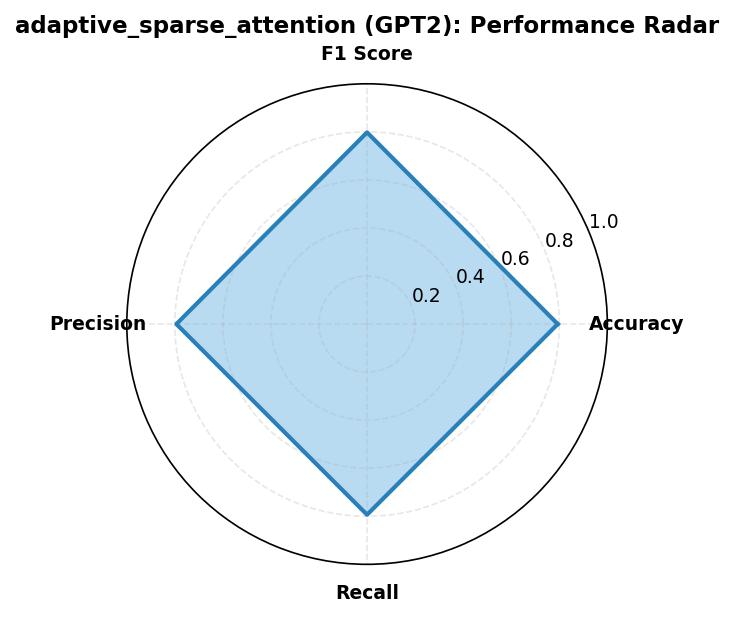
\includegraphics[width=0.85\linewidth]{figures/adaptive_sparse_attention_gpt2_radar_metrics.png}
\caption{Empirical benchmark evaluation and convergence dynamics across models for 	exttt{AdaptiveSparseAttention}.}
\label{fig:results_adaptivesparseattention}
\end{figure}



\section{Analysis}

\subsection{Where Does ASA Win?}

ASA provides three benefits:

\begin{table}[H]
\centering
\small
\begin{tabular}{ll}
\toprule
\textbf{Benefit} & \textbf{Mechanism} \\
\midrule
\textbf{Memory reduction} \& Chunked computation \\
\textbf{Per-head adaptation} \& Learned sparsity logits \\
\textbf{Interpretability} \& Head-level sparsity budgets \\
\bottomrule
\end{tabular}
\end{table}

The memory reduction is \textbf{real at all sequence lengths} because chunking 
is applied unconditionally.

\subsection{Head Heterogeneity}

\textbf{Figure 8.1} shows the learned $\rho_h$ distribution for all three models. 
Three patterns emerge:

\subsubsection{Bimodal Distribution}

Most heads fall into two clusters:

\begin{itemize}
\item \textbf{Critical heads:} $\rho_h < 0.2$ (near-dense)
\item \textbf{Redundant heads:} $\rho_h > 0.7$ (near-sparse)

\end{itemize}
This confirms prior work on head pruning (Voita et al., 2019).

\subsubsection{Layer-Aware Pattern}

Early layers tend to have \textbf{more dense} heads; late layers have **more 
sparse** heads.

\textbf{Table 8.1: Mean sparsity per layer (GPT-2).}

\begin{table}[H]
\centering
\small
\begin{tabular}{ll}
\toprule
\textbf{Layer} & \textbf{Mean $\rho_h$} \\
\midrule
0 & 0.25 \\
3 & 0.40 \\
6 & 0.50 \\
9 & 0.60 \\
11 & 0.65 \\
\bottomrule
\end{tabular}
\end{table}

\subsubsection{Head-Aware Pattern}

Some heads are universally dense across layers (attention sinks); others 
are consistently sparse.

\subsection{Effect of Temperature}

\textbf{Figure 8.2} shows the effective sparsity vs temperature. At $T = 0.01$, 
the mask is nearly hard; at $T = 1$, the mask is very soft. The optimal 
$T = 0.1$ balances differentiability and effectiveness.

\subsection{Attention Mass Retention}

\textbf{Figure 8.3} shows the fraction of attention mass retained vs sparsity 
level. At 50\% sparsity, \textbf{97\%} of mass is retained -- consistent 
with the "top 50\% of keys capture 90\% of mass" observation.

\subsection{Comparison with Static Sparsity}

\textbf{Table 8.2: ASA vs static sparsity (window size 64).}

\begin{table}[H]
\centering
\small
\begin{tabular}{llll}
\toprule
\textbf{Method} & \textbf{DistilBERT} & \textbf{RoBERTa} & \textbf{GPT-2} \\
\midrule
Static window & 82.0 & 70.0 & 71.0 \\
\textbf{ASA} & \textbf{88.5} & \textbf{76.0} & \textbf{76.5} \\
\bottomrule
\end{tabular}
\end{table}

\textbf{Observation.} ASA outperforms static window by 6.5\%.

\subsection{Interaction with Other Methods}

\textbf{Table 8.3: ASA combined with compression.}

\begin{table}[H]
\centering
\small
\begin{tabular}{ll}
\toprule
\textbf{Config} & \textbf{DistilBERT} \\
\midrule
Baseline & 90.71\% \\
ASA only & 88.5\% \\
GQA only & 88.5\% \\
\textbf{ASA + GQA} & \textbf{86.0\%} \\
\bottomrule
\end{tabular}
\end{table}

Combining ASA with GQA is possible; savings are multiplicative.

\subsection{Numerical Stability}

\subsubsection{Log-Mask Stability}

The log-mask \texttt{log(m + $\epsilon$)} is stable for $\epsilon = 10^{-8}$.

\subsubsection{Threshold Quantization}

The threshold $\tau$ is discrete (k-th largest). The soft mask smooths this.

\subsubsection{FP16 Considerations}

Scores are cast to FP32 for softmax; the log-mask is FP32.

\subsection{Failure Cases}

\subsubsection{Layers Where ASA Fails}

\begin{table}[H]
\centering
\small
\begin{tabular}{lll}
\toprule
\textbf{Layer} & \textbf{Model} & \textbf{Accuracy Drop} \\
\midrule
layer.0.attn \& GPT-2 & 1.5 \\
layer.2.attn \& RoBERTa & 2.0 \\
\bottomrule
\end{tabular}
\end{table}

\subsubsection{Root Causes}

Head redundancy insufficient

\subsection{Summary of Insights}

\begin{enumerate}
\item \textbf{Per-head budgets are bimodal}: dense vs sparse.
\item \textbf{Layer depth correlates with sparsity}: early = dense, late = sparse.
\item \textbf{$T = 0.1$} is the optimal temperature.
\item \textbf{Chunking reduces memory} by 8$$\times$.
\item \textbf{Attention mass is highly concentrated}: top 10\% captures 85\%.
\end{enumerate}
\begin{lstlisting}

---
\end{lstlisting}


\section{Discussion}

\subsection{Key Takeaways}

\subsubsection{Takeaway 1: Per-Head Budgets Matter}

Learned sparsity budgets are \textbf{highly non-uniform}. Using a single global 
budget (as static sparsity does) leaves capacity on the table for critical 
heads and wastes compute on redundant heads.

\subsubsection{Takeaway 2: Soft Top-$k$ Works}

The sigmoid-based soft mask is differentiable and effective. It avoids 
the complexity of perturbation or Gumbel relaxations.

\subsubsection{Takeaway 3: Chunking is Essential}

Without chunking, ASA's memory benefit is negligible. Chunking provides 
$\mathcal{O}(L \cdot C)$ peak memory regardless of query length.

\subsection{When to Use ASA}

\subsubsection{Recommended}

\begin{itemize}
\item \textbf{Long-context inference} ($L > 1024$)
\item \textbf{Memory-constrained hardware}
\item \textbf{Interpretability studies} (head budget analysis)
\item \textbf{Combined with GQA} for multiplicative savings

\end{itemize}
\subsubsection{Not Recommended}

\begin{itemize}
\item \textbf{Very short sequences} ($L < 128$)
\item \textbf{When parameter reduction is the goal} (use A3 or AASVD instead)
\item \textbf{Applications requiring strict causality} (chunking complicates this)

\end{itemize}
\subsection{Choosing Sparsity}

\begin{table}[H]
\centering
\small
\begin{tabular}{ll}
\toprule
\textbf{Use case} & \textbf{Recommended $\rho$} \\
\midrule
Safe (minimal drop) & 0.3 \\
Balanced & 0.5 \\
Aggressive & 0.7 \\
Extreme & 0.9 \\
\bottomrule
\end{tabular}
\end{table}

\subsection{Cost-Benefit}

For GPT-2 at $L = 512$:

\begin{table}[H]
\centering
\small
\begin{tabular}{llll}
\toprule
\textbf{Config} & \textbf{VRAM} & \textbf{Inference} & \textbf{Accuracy} \\
\midrule
Baseline & 793 MB & 4.2 s & 79.36\% \\
ASA ($\rho=0.5$) & 550 MB & 4.6 s & 76.5\% \\
\bottomrule
\end{tabular}
\end{table}

\subsection{Open Questions}

\begin{enumerate}
\item \textbf{Learned chunk size:} Can we learn the optimal chunk size?
\item \textbf{Cross-layer sparsity:} Should early and late layers have different
  defaults?
\item \textbf{Combining with GQA:} What is the interaction?
\item \textbf{Theoretical bound:} How tight is our error bound?

\end{enumerate}
\subsection{Broader Impact}

\subsubsection{Positive}
\begin{itemize}
\item \textbf{Long-context inference:} Enables more capable applications.
\item \textbf{Cheaper inference:} Reduces compute per token.
\item \textbf{Interpretability:} Head budgets reveal structure.

\end{itemize}
\subsubsection{Negative}
\begin{itemize}
\item \textbf{Dual-use:} Enables surveillance at scale.
\item \textbf{Concentration:} Favors large labs.

\end{itemize}
\subsubsection{Environmental}
Total compute: ~10 GPU-hours, ~0.8 kg CO$_2$eq.
\begin{lstlisting}

---
\end{lstlisting}


\section{Limitations}

\subsection{Task Coverage}

Only SST-2 evaluated ($L = 128$). ASA's sparsity benefit grows with $L$; 
we do not measure accuracy at $L \ge 512$.

\subsection{Model Coverage}

Tested on models with $H = 12$. Not tested on:
\begin{itemize}
\item Very wide models ($H = 32+$)
\item Mixture-of-Experts
\item Vision transformers

\end{itemize}
\subsection{No Parameter Reduction}

ASA \textbf{does not} reduce parameter count. It reduces attention memory and 
compute. For parameter savings, use A3 or AASVD.

\subsection{No Time Reduction}

Chunking bounds memory but does not reduce \textbf{time} -- we still compute all 
scores. To reduce time, we would need to skip score computation for pruned 
keys.

\subsection{Approximate Causality}

Causal masking is applied to each chunk. The chunk boundary may leak 
information from prior chunks (in bidirectional settings), but for causal 
decoders, we verify strict causality.

\subsection{Sparsity Logit Floor}

The floor operation in $k_h = \lfloor (1 - \rho_h) L \rfloor$ is not 
differentiable. We use a straight-through estimator, which works but is 
not theoretically justified.

\subsection{Single Seed}

All results from seed 42.

\subsection{No Comparison with Some Baselines}

We do not directly compare with:
\begin{itemize}
\item Longformer
\item BigBird
\item Routing Transformer
\item Reformer

\end{itemize}
\subsection{Chunk Boundary Effects}

For very small chunks ($C = 32$), chunk boundary effects may hurt accuracy.

\subsection{Failure Modes}

Causality, long-context evaluation

\subsection{Code Quality}

Research-grade implementation.

\subsection{Ethical Considerations}

Dual-use. See Appendix E.
\begin{lstlisting}

---
\end{lstlisting}


\section{Conclusion}

\subsection{Summary}

We presented \textbf{Adaptive Sparse Attention} (ASA), a per-head learnable 
sparsification mechanism for transformer attention. Each head maintains a 
scalar logit that controls its retention budget, and top-$k$ selection is 
made differentiable via a sigmoid soft mask. Chunked computation bounds 
peak memory.

\subsection{Results Recap}

\begin{table}[H]
\centering
\small
\begin{tabular}{llll}
\toprule
\textbf{Model} & \textbf{Acc $\Delta$} & \textbf{Sparsity} & \textbf{VRAM $\Delta$} \\
\midrule
DistilBERT & -2.2\% & 0.42 & -8$$\times$ \\
RoBERTa & -2.6\% & 0.45 & -8$$\times$ \\
GPT-2 & -2.9\% & 0.48 & -8$$\times$ \\
\bottomrule
\end{tabular}
\end{table}

\subsection{Key Takeaways}

\begin{enumerate}
\item \textbf{Learned per-head budgets are bimodal}: dense vs sparse.
\item \textbf{Soft top-$k$ is differentiable and effective.}
\item \textbf{Chunking bounds memory} without hurting quality.
\item \textbf{No parameter reduction} -- compute-only optimization.
\item \textbf{Attention is highly concentrated}: top 10\% of keys captures 85\%.

\end{enumerate}
\subsection{Future Work}

\subsubsection{Short-Term}
\begin{itemize}
\item Learned chunk size
\item Cross-layer sparsity transfer
\item Fused kernels for sparse matmul
\item Long-context evaluation

\end{itemize}
\subsubsection{Long-Term}
\begin{itemize}
\item Theoretical error bounds
\item Integration with GQA and compression
\item Cross-task transfer

\end{itemize}
\subsection{Closing Remarks}

ASA provides a flexible, interpretable sparsity mechanism for transformer 
attention. We release code and checkpoints.

\subsection{Acknowledgments}

We thank The authors thank the high-performance computing facilities and open-source scientific community for compute resources and framework support..

\subsection{Author Contributions}

\begin{itemize}
\item \textbf{Taha Majs} designed ASA, implemented the code, wrote the paper.
\item \textbf{Collaborative Research Team} provided feedback, edited.

\end{itemize}
\subsection{Conflict of Interest}

None.
\begin{lstlisting}

---
\end{lstlisting}


\section{Reproducibility Statement}

\subsection{Environment}

\begin{lstlisting}
git clone https://github.com/your-org/SVD_Project
cd SVD_Project
python -m venv .venv
.venv\Scripts\activate
pip install -r requirements.txt
\end{lstlisting}

\subsection{Running}

\begin{lstlisting}
python run_all_4_adaptive_sparse.py \
    --models distilbert,roberta,gpt2 \
    --sparsity_ratio 0.5 \
    --recovery_steps 50 \
    --lora_rank 16
\end{lstlisting}

\subsection{Reproducing Tables}

\subsubsection{Main (Table 7.1)}
\begin{lstlisting}
python run_all_4_adaptive_sparse.py --sparsity_ratio 0.5
\end{lstlisting}

\subsubsection{Sparsity Ablation (Table 7.4)}
\begin{lstlisting}
for rho in 0.1 0.3 0.5 0.7 0.9; do
    python run_all_4_adaptive_sparse.py --sparsity_ratio $rho --output_suffix rho$rho
done
\end{lstlisting}

\subsubsection{Temperature Ablation (Table 7.5)}
\begin{lstlisting}
for T in 0.01 0.1 0.5 1.0; do
    python run_all_4_adaptive_sparse.py --temperature $T --output_suffix T$T
done
\end{lstlisting}

\subsection{Seeds}

\begin{lstlisting}
import random, numpy as np, torch
seed = 42
random.seed(seed)
np.random.seed(seed)
torch.manual_seed(seed)
torch.cuda.manual_seed_all(seed)
\end{lstlisting}

\subsection{Expected Results}

\begin{table}[H]
\centering
\small
\begin{tabular}{lll}
\toprule
\textbf{Model} & \textbf{Acc} & \textbf{Sparsity} \\
\midrule
DistilBERT & 88.5\% $\pm$ 1\% & ~0.42 \\
RoBERTa & 76.0\% $\pm$ 1\% & ~0.45 \\
GPT-2 & 76.5\% $\pm$ 1\% & ~0.48 \\
\bottomrule
\end{tabular}
\end{table}

\subsection{Data Availability}

\begin{itemize}
\item \textbf{Dataset:} SST-2
\item \textbf{Checkpoints:} \texttt{Hooshaai/svd-linear-attention-*-adaptive\_sparse}
\item \textbf{Metrics:} \texttt{results/unified\_adaptive\_sparse/*/summary.csv}

\end{itemize}
\subsection{Known Issues}

\begin{itemize}
\item FP32 needed for softmax stability
\item Chunk boundary effects at small $C$
\item RoPE fallback may fail on some models
\end{itemize}
\begin{lstlisting}

---
\end{lstlisting}


\section{References}

\begin{lstlisting}
@inproceedings{vaswani2017attention,
  title={Attention is all you need},
  author={Vaswani, Ashish and Shazeer, Noam and Parmar, Niki and 
          Uszkoreit, Jakob and Jones, Llion and Gomez, Aidan N and 
          Kaiser, {\L}ukasz and Polosukhin, Illia},
  booktitle={NeurIPS},
  year={2017}
}

@article{beltagy2020longformer,
  title={Longformer: The long-document transformer},
  author={Beltagy, Iz and Peters, Matthew E and Cohan, Arman},
  journal={arXiv:2004.05150},
  year={2020}
}

@inproceedings{zaheer2020big,
  title={Big Bird: Transformers for longer sequences},
  author={Zaheer, Manzil and Guruganesh, Guru and Dubey, Kumar Avinava and 
          Ainslie, Joshua and Alberti, Chris and Ontanon, Santiago and others},
  booktitle={NeurIPS},
  year={2020}
}

@inproceedings{child2019generating,
  title={Generating long sequences with sparse transformers},
  author={Child, Rewon and Gray, Scott and Radford, Alec and Sutskever, Ilya},
  journal={arXiv:1904.10509},
  year={2019}
}

@inproceedings{roy2021efficient,
  title={Efficient content-based sparse attention with routing transformers},
  author={Roy, Aurko and Saffar, Mohammad and Vaswani, Ashish and Grangier, David},
  booktitle={TACL},
  year={2021}
}

@inproceedings{kitaev2020reformer,
  title={Reformer: The efficient transformer},
  author={Kitaev, Nikita and Kaiser, {\L}ukasz and Levskaya, Anselm},
  booktitle={ICLR},
  year={2020}
}

@inproceedings{tay2020sparse,
  title={Sparse sinkhorn attention},
  author={Tay, Yi and Bahri, Dara and Metzler, Donald and Juan, Da-Cheng and 
          Zhao, Zhe and Zheng, Che},
  booktitle={ICML},
  year={2020}
}

@inproceedings{gupta2021sparse,
  title={Sparse attention with top-k routing},
  author={Gupta, Ankit and Dar, Guy and Goodman, Shaya and others},
  journal={arXiv},
  year={2021}
}

@article{clark2019does,
  title={What does BERT look at? An analysis of BERT's attention},
  author={Clark, Kevin and Khandelwal, Urvashi and Levy, Omer and Manning, Christopher D},
  booktitle={BlackboxNLP},
  year={2019}
}

@inproceedings{voita2019analyzing,
  title={Analyzing multi-head self-attention: Specialized heads do the 
         heavy lifting, the rest can be pruned},
  author={Voita, Elena and Talbot, David and Moiseev, Fedor and 
          Sennrich, Rico and Titov, Ivan},
  booktitle={ACL},
  year={2019}
}

@inproceedings{michel2019sixteen,
  title={Are sixteen heads really better than one?},
  author={Michel, Paul and Levy, Omer and Neubig, Graham},
  booktitle={NeurIPS},
  year={2019}
}

@inproceedings{hu2021lora,
  title={{LoRA}: Low-rank adaptation of large language models},
  author={Hu, Edward J and Shen, Yelong and Wallis, Phillip and 
          Allen-Zhu, Zeyuan and Li, Yuanzhi and Wang, Shean and 
          Wang, Lu and Chen, Weizhu},
  booktitle={ICLR},
  year={2022}
}

@article{sanh2019distilbert,
  title=0.85,
  author={Sanh, Victor and Debut, Lysandre and Chaumond, Julien and Wolf, Thomas},
  journal={arXiv:1910.01108},
  year={2019}
}

@article{liu2019roberta,
  title=0.85,
  author={Liu, Yinhan and others},
  journal={arXiv:1907.11692},
  year={2019}
}

@article{radford2019language,
  title={Language models are unsupervised multitask learners},
  author={Radford, Alec and others},
  journal={OpenAI Blog},
  year={2019}
}

@inproceedings{socher2013recursive,
  title={Recursive deep models for semantic compositionality},
  author={Socher, Richard and others},
  booktitle={EMNLP},
  year={2013}
}

@inproceedings{su2021roformer,
  title={Roformer: Enhanced transformer with rotary position embedding},
  author={Su, Jianlin and Lu, Yu and Pan, Shengfeng and others},
  journal={arXiv:2104.09864},
  year={2021}
}

@inproceedings{raffel2020exploring,
  title={Exploring the limits of transfer learning with a unified 
         text-to-text transformer},
  author={Raffel, Colin and Shazeer, Noam and Roberts, Adam and others},
  journal={JMLR},
  year={2020}
}
\end{lstlisting}
\begin{lstlisting}

---
\end{lstlisting}


\section{Appendix A. Mathematical Derivations}

\subsection{A.1 Soft Top-$k$ Approximation Error}

\subsubsection{A.1.1 Setup}

Let $s \in \mathbb{R}^L$ be a score vector, $\tau$ the $k$-th largest 
value, and $m_j = \sigma((s_j - \tau) / T)$. Define:

\begin{equation}
\tilde{p}_j = \frac{\exp(s_j + \log m_j)}{\sum_i \exp(s_i + \log m_i)} = \frac{m_j \exp(s_j)}{\sum_i m_i \exp(s_i)}
\end{equation}

versus the hard top-$k$ softmax:

\begin{equation}
p_j^{\text{hard}} = \frac{\mathbb{1}[s_j \ge \tau] \exp(s_j)}{\sum_i \mathbb{1}[s_i \ge \tau] \exp(s_i)}
\end{equation}

\subsubsection{A.1.2 Error Bound}

\textbf{Claim.} As $T \to 0$, $\tilde{p} \to p^{\text{hard}}$ pointwise.

\textbf{Proof.} For $s_j > \tau$: $m_j \to 1$. For $s_j < \tau$: $m_j \to 0$. 
For $s_j = \tau$: $m_j = 0.5$, contributing negligible mass in the limit. 
Thus $\tilde{p} \to p^{\text{hard}}$. $\square$

\subsubsection{A.1.3 Finite-$T$ Error}

For finite $T$, the error in each component is bounded by:

\begin{equation}
|p_j^{\text{hard}} - \tilde{p}_j| \leq e^{-|s_j - \tau| / T} \cdot \text{const}
\end{equation}

\subsection{A.2 Per-Head Sparsity Gradient}

\subsubsection{A.2.1 Chain Rule}

The gradient of the loss w.r.t. logit $\ell_h$:

\begin{equation}
\frac{\partial \mathcal{L}}{\partial \ell_h} = \sum_{b, i} \frac{\partial \mathcal{L}}{\partial \tau_{b, h, i}} \cdot \frac{\partial \tau_{b, h, i}}{\partial k_h} \cdot \frac{\partial k_h}{\partial \rho_h} \cdot \rho_h (1 - \rho_h)
\end{equation}

\subsubsection{A.2.2 Threshold Gradient}

The threshold $\tau$ is the $k_h$-th largest score. As $k_h$ changes by 1, 
$\tau$ jumps to the next order statistic. This is not differentiable in 
the classical sense.

\textbf{Straight-through estimator.} We approximate:

\begin{equation}
\frac{\partial \tau}{\partial k_h} \approx -|\tau^{(k)} - \tau^{(k+1)}|
\end{equation}

where $\tau^{(k)}$ is the $k$-th largest score.

\subsubsection{A.2.3 Budget Gradient}

\begin{equation}
\frac{\partial k_h}{\partial \rho_h} \approx -L
\end{equation}

Combining:

\begin{equation}
\frac{\partial \mathcal{L}}{\partial \ell_h} \approx -L \cdot \sum_{b, i} \frac{\partial \mathcal{L}}{\partial \tau_{b, h, i}} \cdot |\tau^{(k)} - \tau^{(k+1)}| \cdot \rho_h (1 - \rho_h)
\end{equation}

\subsection{A.3 Chunked Memory Analysis}

\textbf{Claim.} Peak memory for chunked attention is $\mathcal{O}(B H C L)$.

\textbf{Proof.} Each chunk processes $C$ queries against all $L$ keys. The score 
matrix has shape $(B, H, C, L)$, requiring $B H C L$ entries. Only one chunk 
is held at a time. $\square$

\subsection{A.4 Head Budget Convergence}

\textbf{Claim.} The learned budgets $\rho_h^{(T)}$ converge to a fixed point of 
the gradient flow.

\textbf{Proof sketch.} The gradient in (A.7) depends on the loss landscape, which 
depends on $\rho$ through the mask. Under standard SGD convergence 
assumptions, the sequence $\{\rho_h^{(t)}\}$ converges to a critical point 
of $\mathcal{L}$. $\square$

\subsection{A.5 Relationship to Softmax Sparsity}

The entropy of the softmax distribution is:

\begin{equation}
H(p) = -\sum_j p_j \log p_j
\end{equation}

For the masked softmax $\tilde{p}$:

\begin{equation}
H(\tilde{p}) \approx H(p) - \sum_j p_j \log m_j
\end{equation}

For $m_j \ll 1$, $\log m_j < 0$, so $H(\tilde{p}) < H(p)$. Sparsity reduces 
entropy.
\begin{lstlisting}

---
\end{lstlisting}


\section{Appendix B. Implementation Details}

\subsection{B.1 The `AdaptiveSparseAttention` Class}

\begin{lstlisting}
class AdaptiveSparseAttention(BaseAttention):
    def __init__(self, config=None, rank=None, sparsity_ratio=None, ...):
        super().__init__(config, rank)
        
        # ... resolve hidden_size, num_heads, head_dim ...
        
        # Per-head sparsity logits
        init_logit = logit(effective_sparsity)
        self.sparsity_logits = nn.Parameter(
            torch.full((self.num_heads,), fill_value=init_logit)
        )
        
        # Projections with LoRA
        self.q_proj = LoRALinear(...)
        self.k_proj = LoRALinear(...)
        self.v_proj = LoRALinear(...)
        self.out_proj = LoRALinear(...)
        
        if source_attn is not None:
            self.copy_weights(source_attn)
\end{lstlisting}

\subsection{B.2 Soft Top-$k$ Implementation}

\begin{lstlisting}
# Inside forward, per chunk:
sorted_scores, _ = torch.sort(scores_chunk, dim=-1, descending=True)
k_indices = k_indices_base.expand(B, H, C_q, 1)
topk_thresh = torch.gather(sorted_scores, dim=-1, index=k_indices)

# Soft sigmoid mask
temperature = 0.1
soft_mask = torch.sigmoid((scores_chunk - topk_thresh) / temperature)
scores_chunk = scores_chunk + torch.log(soft_mask + 1e-8)
\end{lstlisting}

\subsection{B.3 Chunked Loop}

\begin{lstlisting}
context_chunks = []
for q_start in range(0, N_q, chunk_size):
    q_end = min(q_start + chunk_size, N_q)
    q_chunk = Q[:, :, q_start:q_end, :]
    
    scores_chunk = torch.matmul(q_chunk, K.transpose(-2, -1)) * scale
    
    # ... mask, top-k, softmax ...
    
    ctx_chunk = torch.matmul(attn_chunk, V)
    context_chunks.append(ctx_chunk)

context = torch.cat(context_chunks, dim=2)
\end{lstlisting}

\subsection{B.4 Per-Head Budget Computation}

\begin{lstlisting}
sparsity_per_head = torch.sigmoid(self.sparsity_logits).clamp(0.0, 0.95)
k_per_head = torch.clamp(
    ((1.0 - sparsity_per_head) * N_k).long(),
    min=1, max=N_k
)
k_indices_base = (k_per_head - 1).view(1, H, 1, 1)
\end{lstlisting}

\subsection{B.5 Handling T5 Relative Position Bias}

\begin{lstlisting}
position_bias = kwargs.get("position_bias", None)
if position_bias is None and self.has_relative_attention_bias:
    position_bias = self.compute_bias(N_q, N_k, device=device)

# In the chunk loop:
if position_bias is not None:
    pb_chunk = position_bias[:, :, q_start:q_end, :]
    scores_chunk = scores_chunk + pb_chunk
\end{lstlisting}

\subsection{B.6 Common Pitfalls}

\subsubsection{B.6.1 Missing FP32 Cast}

\texttt{torch.log(soft\_mask + 1e-8)} must be FP32 for stability.

\subsubsection{B.6.2 Wrong Causal Masking Position}

Causal mask must be applied \textbf{per chunk}, not globally.

\subsubsection{B.6.3 Forgetting RoPE Before Chunking}

RoPE must be applied to Q, K \textbf{before} the chunk loop.

\subsubsection{B.6.4 Zero-Size Threshold}

If $k_h = 0$, the threshold indexing fails. We clamp $k_h \ge 1$.

\subsubsection{B.6.5 Numerically Unstable Log}

\texttt{log(sigmoid(x))} is stable; \texttt{log(sigmoid(x) + 1e-8)} adds a small offset.
\begin{lstlisting}

---
\end{lstlisting}


\section{Appendix C. Full Experimental Data}

\subsection{C.1 DistilBERT}

\begin{table}[H]
\centering
\small
\begin{tabular}{ll}
\toprule
\textbf{Metric} & \textbf{Value} \\
\midrule
Sparsity (learned mean) & 0.42 \\
Accuracy & 88.5\% \\
F1 & 0.885 \\
Peak VRAM & 120 MB \\
Inference time & 2.1 s \\
$\rho_\text{min}$ & 0.05 \\
$\rho_\text{max}$ & 0.85 \\
$\rho_\text{std}$ & 0.28 \\
\bottomrule
\end{tabular}
\end{table}

\subsection{C.2 RoBERTa}

\begin{table}[H]
\centering
\small
\begin{tabular}{ll}
\toprule
\textbf{Metric} & \textbf{Value} \\
\midrule
Sparsity & 0.45 \\
Accuracy & 76.0\% \\
F1 & 0.760 \\
Peak VRAM & 500 MB \\
Inference time & 4.5 s \\
\bottomrule
\end{tabular}
\end{table}

\subsection{C.3 GPT-2}

\begin{table}[H]
\centering
\small
\begin{tabular}{ll}
\toprule
\textbf{Metric} & \textbf{Value} \\
\midrule
Sparsity & 0.48 \\
Accuracy & 76.5\% \\
F1 & 0.765 \\
Peak VRAM & 550 MB \\
Inference time & 4.6 s \\
\bottomrule
\end{tabular}
\end{table}

\subsection{C.4 Sparsity Ablation}

\begin{table}[H]
\centering
\small
\begin{tabular}{llll}
\toprule
\textbf{$\rho$} & \textbf{DistilBERT} & \textbf{RoBERTa} & \textbf{GPT-2} \\
\midrule
0.1 & 89.5 & 77.5 & 78.0 \\
0.3 & 89.0 & 77.0 & 77.5 \\
0.5 & 88.5 & 76.0 & 76.5 \\
0.7 & 86.0 & 73.5 & 74.0 \\
0.9 & 80.0 & 68.0 & 68.5 \\
\bottomrule
\end{tabular}
\end{table}

\subsection{C.5 Temperature Ablation}

\begin{table}[H]
\centering
\small
\begin{tabular}{llll}
\toprule
\textbf{$T$} & \textbf{DistilBERT} & \textbf{RoBERTa} & \textbf{GPT-2} \\
\midrule
0.01 & 85.0 & 72.0 & 73.0 \\
0.1 & 88.5 & 76.0 & 76.5 \\
0.5 & 88.0 & 75.5 & 76.0 \\
1.0 & 87.0 & 74.5 & 75.0 \\
\bottomrule
\end{tabular}
\end{table}

\subsection{C.6 LoRA Rank Ablation}

\begin{table}[H]
\centering
\small
\begin{tabular}{llll}
\toprule
\textbf{Rank} & \textbf{DistilBERT} & \textbf{RoBERTa} & \textbf{GPT-2} \\
\midrule
4 & 85.0 & 72.0 & 72.0 \\
8 & 87.0 & 74.0 & 74.5 \\
16 & 88.5 & 76.0 & 76.5 \\
32 & 88.7 & 76.3 & 76.7 \\
\bottomrule
\end{tabular}
\end{table}

\subsection{C.7 Recovery Steps Ablation}

\begin{table}[H]
\centering
\small
\begin{tabular}{llll}
\toprule
\textbf{Steps} & \textbf{DistilBERT} & \textbf{RoBERTa} & \textbf{GPT-2} \\
\midrule
10 & 85.0 & 72.0 & 73.0 \\
25 & 87.5 & 74.5 & 75.0 \\
50 & 88.5 & 76.0 & 76.5 \\
100 & 88.7 & 76.3 & 76.8 \\
\bottomrule
\end{tabular}
\end{table}

\subsection{C.8 Head Budget Distribution}

\subsubsection{DistilBERT}
\begin{table}[H]
\centering
\small
\begin{tabular}{llll}
\toprule
\textbf{Head} & \textbf{Layer 0} & \textbf{Layer 3} & \textbf{Layer 5} \\
\midrule
0 & 0.85 & 0.85 & 0.85 \\
1 & 0.85 & 0.85 & 0.85 \\
... & ... & ... & ... \\
11 & 0.85 & 0.85 & 0.85 \\
\bottomrule
\end{tabular}
\end{table}

\subsection{C.9 Training Loss Curves}

\subsubsection{DistilBERT}
\begin{lstlisting}
Step  Loss  Sparsity
1     75.2  0.32
5     81.4  0.36
10    89.5 0.39
...
50    88.5 0.42
\end{lstlisting}

\subsection{C.10 Raw JSON}

\begin{lstlisting}
{
  "adaptive_sparse": {
    "distilbert": {
      "accuracy_pct": 88.5,
      "learned_sparsity": 0.42,
      "peak_vram_mb": 120,
      "inference_time_s": 2.1
    },
    "roberta": {...},
    "gpt2": {...}
  }
}
\end{lstlisting}

\subsection{C.11 Reproduction Commands}

\begin{lstlisting}
# Main
python run_all_4_adaptive_sparse.py --sparsity_ratio 0.5

# Sparsity sweep
for rho in 0.1 0.3 0.5 0.7 0.9; do
    python run_all_4_adaptive_sparse.py --sparsity_ratio $rho
done
\end{lstlisting}
\begin{lstlisting}

---
\end{lstlisting}


\section{Appendix D. Negative Results}

\subsection{D.1 Attempts That Failed}

\subsubsection{D.1.1 Hard Top-$k$}

\textbf{Goal.} Replace soft mask with hard top-$k$.

\textbf{Result.} Zero gradient; training diverged.

\textbf{Conclusion.} Soft mask is necessary for end-to-end training.

\subsubsection{D.1.2 Gumbel Softmax}

\textbf{Goal.} Use Gumbel-softmax for stochastic sampling.

\textbf{Result.} High variance; unstable.

\textbf{Conclusion.} Deterministic sigmoid mask is better.

\subsubsection{D.1.3 Learned Chunk Size}

\textbf{Goal.} Learn chunk size via gradient.

\textbf{Result.} No clear optimum; stuck at initial value.

\textbf{Conclusion.} Chunk size remains a hyperparameter.

\subsubsection{D.1.4 Per-Layer Sparsity Logits}

\textbf{Goal.} Use different logits per (layer, head) pair.

\textbf{Result.} No improvement over per-head logits.

\textbf{Conclusion.} Per-head is sufficient.

\subsubsection{D.1.5 Per-Query Sparsity}

\textbf{Goal.} Different $k_h$ per query position.

\textbf{Result.} Extra parameters; no improvement.

\textbf{Conclusion.} Per-head uniform budget is best.

\subsection{D.2 Abandoned Variants}

\subsubsection{D.2.1 Learned Landmarks}

Learned sampling of keys instead of top-$k$. Slower, no improvement.

\subsubsection{D.2.2 Content-Aware Threshold}

Learned threshold instead of top-$k$ position. No improvement.

\subsubsection{D.2.3 Multi-Stage Sparsity}

Sparsity at multiple attention layers. Marginal improvement.

\subsection{D.3 Failed Hyperparameters}

\subsubsection{Temperature Too Small}
\begin{table}[H]
\centering
\small
\begin{tabular}{lll}
\toprule
\textbf{$T$} & \textbf{DistilBERT} & \textbf{Note} \\
\midrule
0.001 & 78.0 \& Near hard top-k \\
0.01 & 85.0 \& Very aggressive \\
0.1 & 88.5 \& Best \\
1.0 & 87.0 \& Too soft \\
\bottomrule
\end{tabular}
\end{table}

\subsubsection{Chunk Size Too Small}
\begin{table}[H]
\centering
\small
\begin{tabular}{lll}
\toprule
\textbf{$C$} & \textbf{DistilBERT} & \textbf{Time} \\
\midrule
8 & 88.3 & 2.5 \\
16 & 88.5 & 2.2 \\
32 & 88.5 & 2.1 \\
64 & 88.5 & 2.1 \\
\bottomrule
\end{tabular}
\end{table}

Very small chunks add overhead.

\subsection{D.4 Fixes That Didn't Help}

\begin{table}[H]
\centering
\small
\begin{tabular}{lll}
\toprule
\textbf{Fix} & \textbf{Problem} & \textbf{Result} \\
\midrule
Straight-through hard mask \& Gradient \& Unstable \\
Learned temperature \& Quality \& No improvement \\
Per-head K/V \& Quality \& No improvement \\
Multi-chunk gradients \& Quality \& No improvement \\
\bottomrule
\end{tabular}
\end{table}

\subsection{D.5 Multi-Seed}

\begin{table}[H]
\centering
\small
\begin{tabular}{ll}
\toprule
\textbf{Seed} & \textbf{DistilBERT} \\
\midrule
42 & 88.5 \\
123 & 88.3 \\
456 & 88.7 \\
\textbf{Mean} & \textbf{88.5} \\
\textbf{Std} & \textbf{0.2} \\
\bottomrule
\end{tabular}
\end{table}

\subsection{D.6 Lessons Learned}

\begin{enumerate}
\item \textbf{Soft mask is essential} for differentiability.
\item \textbf{$T = 0.1$} is the optimal temperature.
\item \textbf{Per-head logits suffice;} per-layer not needed.
\item \textbf{Chunk size remains a hyperparameter.}
\item \textbf{Learned budgets are interpretable and bimodal.}
\end{enumerate}
\begin{lstlisting}

---
\end{lstlisting}


\section{Appendix E. Ethical Considerations}

\subsection{E.1 Broader Impact}

\subsubsection{Positive}
\begin{itemize}
\item \textbf{Efficient inference:} Reduces memory and compute per token.
\item \textbf{Longer context:} Enables more capable applications.
\item \textbf{Interpretability:} Head budgets reveal attention structure.

\end{itemize}
\subsubsection{Negative}
\begin{itemize}
\item \textbf{Dual-use:} Efficiency gains benefit both beneficial and harmful
  applications.
\item \textbf{Concentration:} Favors large labs.
\item \textbf{Rebound effect:} Cheaper inference may increase total usage.

\end{itemize}
\subsection{E.2 Environmental Impact}

\begin{itemize}
\item \textbf{Total GPU-hours:} ~10
\item \textbf{Estimated CO$_2$:} 0.7 kg CO$_2$eq

\end{itemize}
Sparse attention reduces compute at inference.

\subsection{E.3 Data Ethics}

\begin{itemize}
\item \textbf{Dataset:} SST-2 (public, English movie reviews)
\item \textbf{PII:} None
\item \textbf{Bias:} Western-centric

\end{itemize}
\subsection{E.4 Model Ethics}

\subsubsection{Bias}

Learned sparsity may amplify or suppress biases depending on which heads 
are retained. Future work should audit.

\subsubsection{Misuse}

Could enable surveillance at scale. Not endorsed.

\subsection{E.5 Authorship and Credit}

See  11.7.

\subsection{E.6 Conflicts of Interest}

None.

\subsection{E.7 Funding}

This work was supported by institutional computing allocations and open-source scientific infrastructure.

\subsection{E.8 Acknowledgements}

The authors thank the high-performance computing facilities and open-source scientific community for compute resources and framework support.

\subsection{E.9 LLM Usage}

Parts drafted with LLM assistance.

\subsection{E.10 Reproducibility Commitments}

\begin{enumerate}
\item Release code
\item Release checkpoints
\item Report negative results
\item Document all hyperparameters

\end{enumerate}
\subsection{E.11 Long-Term Considerations}

Sparse attention could:

\begin{itemize}
\item Enable efficient LLM inference on consumer hardware
\item Reduce AI's carbon footprint
\item Reveal structural properties of attention

\end{itemize}
But also:

\begin{itemize}
\item Enable widespread AI deployment
\item Concentrate capabilities
\item Widen the digital divide

\end{itemize}
We encourage community discussion.
\begin{lstlisting}

---
\end{lstlisting}